\newpage
\chapter{Implementation}
After the design has been specified, the extension's implementation may begin. This section describes further explanation from \autoref{technologies_used} for the technology used. Because no backend implementation is required for the project, this section will only cover the front-end implementation.

\section{User Interface}
This section goes through some of the technical aspects of the user interface of the extension. The user interface was built with React. As described in \autoref{react}, React makes it easy to create interactive UIs. Using JSX makes it even simpler for web designers to change the browser's DOM using HTML. Furthermore, the user interface is developed in TypeScript rather than regular JavaScript to ensure type safety.

\subsection{Build Tool}
Nowadays, most front end projects use a build tool to assist in the development of web applications. The build tool for the user interface is \emph{Webpack 5}\footnote{\emph{Webpack} is a static module bundler for modern JavaScript applications. Webpack version 5 includes faster builds with persistent caching, smaller bundler size, Module Federation, etc. More information on \url{https://webpack.js.org/blog/2020-10-10-webpack-5-release/}}.

\subsection{Component Library}
A component library is used in this project to speed up UI development. The rebass component library is used in this project. \emph{Rebass}\footnote{\emph{Rebass} is a simple React UI component library that allows you to create primitive UI components using the Styled System library. More information on \url{https://rebassjs.org/}} was chosen because it is lightweight and an excellent choice for prototype and UI development without the need to invest time in establishing a custom design system from the start.

\subsection{Code Style}
In this project, a code formatter (Prettier) and linter (ESLint) are used to ensure a uniform code style and conform with TypeScript best practices.

\section{File structure}
This section walks through the project's file structure, as shown in \autoref{directory_tree} \texttt{.husky} is used to format code with prettier on git commit. Webpack generates the \texttt{dist} folder. This folder contains the JavaScript files generated by TypeScript (such as \texttt{background.js}, \texttt{contentScript.js}, \texttt{popup.html}, etc.). From the folder structure it is conceivable that \texttt{yarn} is the package manager and \texttt{jest} is the testing library. The extension's essential files are inside \texttt{src} and \texttt{static}.

\begin{figure}[H]
  \dirtree{%
    .1 /.
    .2 .husky.
    .2 dist.
    .2 src.
    .3 background.
    .4 index.ts.
    .3 components.
    .3 content-script.
    .4 index.ts.
    .3 contexts.
    .4 parameter.tsx.
    .4 pathname.tsx.
    .4 url.tsx.
    .3 options.
    .4 index.css.
    .4 index.tsx.
    .4 options.tsx.
    .3 popup.
    .4 index.css.
    .4 index.tsx.
    .4 popup-with-router.tsx.
    .4 popup.tsx.
    .3 spec.
    .3 types.
    .4 entry-type.ts.
    .3 utils.
    .4 storage.ts.
    .4 tabs.ts.
    .4 url.ts.
    .2 static.
    .3 icons.
    .3 manifest.json.
    .2 webpack.
    .2 .gitignore.
    .2 jest.config.js.
    .2 package.json.
    .2 README.md.
    .2 tsconfig.json.
    .2 yarn.lock.
  }
  \caption{Directory Tree}
  \label{directory_tree}
\end{figure}

\section{Installation}
When a Chrome extension is installed, a manifest file is read, which acts as a contract between the extension and the browser. In addition to trivial data such as the extension's name, description and version, the runtime permissions are defined (\texttt{permissions}). Furthermore, the functions that are to be triggered after events occur are registered with the help of so-called service workers (\texttt{background}). Furthermore, an options page or configuration page (\verb;options_page;) can be defined. The version of the manifest file is determined by \verb;manifest_version;, which is the latest and recommended version at the moment. \texttt{action} allow the user to customize the appearance and behaviour of the buttons that appear on the Chrome toolbar. In this case when the button with the icon \texttt{icons/icon-filtre-16.png} is clicked Chrome will load the \texttt{popup.html} file. Scripts that are statically declared are registered in the manifest under the \verb;content_scripts; field:
\begin{itemize}
  \item \texttt{matches}: Specifies which pages this content script will be injected into. The special pattern that is used \verb;<all_urls>; matches any URL that starts with a permitted scheme\footnote{\texttt{http}, \texttt{https}, \texttt{urn}, \texttt{file}, or \texttt{ftp}, and that can contain "*" characters are all permitted schemes of a URL}.
  \item \texttt{js}: The list of JavaScript files to be injected into matching pages. These are injected in the order they appear in this array.
  \item \verb;run_at;: Controls when JavaScript files are injected into the web page.
\end{itemize}

By setting the \verb;run_at; field to be \verb;document_idle;, the browser chooses a time to inject scripts between \verb;document_end; and immediately after the \emph{window.onload}\footnote{\emph{window.onload} event is fired when the whole page has loaded, including all dependent resources such as stylesheets and images. More information on \url{https://developer.mozilla.org/en-US/docs/Web/API/Window/load_event}} event fires. The exact moment of injection depends on how complex the document is and how long it is taking to load, and is optimized for page load speed \autocite{chrome2021runtime}.

\begin{lstlisting}[language=json, caption={Manifest File (JSON)}, label={lst:manifest}]
{
  "name": "Filtre",
  "description": "A filtering assistant for Chrome",
  "version": "0.1.0",
  "manifest_version": 3,
  "icons": {
    "16": "icons/icon-filtre-16.png",
    "48": "icons/icon-filtre-48.png",
    "128": "icons/icon-filtre-128.png"
  },
  "action": {
    "default_popup": "popup.html",
    "default_title": "Filtre",
    "default_icon": "icons/icon-filtre-16.png"
  },
  "permissions": ["storage", "tabs", "unlimitedStorage"],
  "options_page": "options.html",
  "background": {
    "service_worker": "background.js"
  },
  "content_scripts": [
    {
      "matches": ["<all_urls>"],
      "js": ["contentScript.js"],
      "run_at": "document_idle"
    }
  ]
}
\end{lstlisting}

The function below (\autoref{lst:background}) is fired when the extension is first installed, when the extension is updated to a new version, and when Chrome is updated to a new version. An empty object is set as the initial filters and a default config object is set as the initial configuration.

\begin{lstlisting}[style=ES6, caption={On install functions (TypeScript)}, label={lst:background}]
  import { setStoredConfig, setStoredFilters } from '../utils/storage'

  chrome.runtime.onInstalled.addListener(() => {
    setStoredFilters({})
    setStoredConfig({ excludedParameters: [] })
  })
\end{lstlisting}

\begin{lstlisting}[style=ES6, caption={Helper functions for Chrome Storage API (TypeScript)}]
export const setStoredKey = (
  key: LocalStorageKeys,
  data: Record<string, any>
): Promise<void> => {
  const vals: LocalStorage = { [key]: data }
  return new Promise((resolve) => {
    chrome.storage.local.set(vals, resolve)
  })
}

export const setStoredFilters = (
  filters: Record<string, any>
): Promise<void> => {
  return setStoredKey('filters', filters)
}
\end{lstlisting}

\begin{lstlisting}[style=ES6, caption={TypeScript interface of a LocalStorage object (TypeScript)}]
export interface LocalStorage {
  filters?: Record<string, any>
  config?: Record<string, any>
}

export type LocalStorageKeys = keyof LocalStorage
\end{lstlisting}

\section{Realization}
While the implementation itself was primarily focused on storing records, several issues arose during the process of integrating the source code into a Google Chrome extension that required attention. The primary questions were when and how the URL should be stored. This section discusses the solutions to these issues.

\subsection*{Storing Point in Time}
The first question is addressed by \autoref{lst:manifest}, on the \verb;content_scripts; field. Since the \verb;run_at; field is set to \verb;document_idle;, the URL is stored immediately after the whole page has loaded. That is, everytime a website is viewed or refreshed, the record is always saved, even if the user navigates away from the tab while the page loads.

\subsection*{TypeScript type of data}
To answer the second question, the record that we want to store needs to be uniform. A TypeScript type is created to provide a clear record structure.

\begin{lstlisting}[style=es6, caption={TypeScript type of a record entry (TypeScript)}]
export type ParameterType = {
  uuid: string
  createdAt: number
  version: string
  paramKey: string
  paramValue: string
  count: number
  lastUpdatedAt: number
}

export type Parameters = ParameterType[]

export type PathType = {
  name: string
  subpaths: PathType[]
  parameters: Parameters
}

export type Paths = PathType[]

export type Entry = {
  [host: string]: Paths
}
\end{lstlisting}

\subsection*{Filters in URLs}
As mentioned in \autoref{url_anatomy}, a URL consists of various components, some of which are host name, path and query string. The topics, filters and facets, were also discussed in \autoref{filters_and_facets}. These definitions play an important role when adding persistent filters on a website.

Classic filters are usually placed in the path of a URL because it is hierarchical. Meanwhile, facets typically use the query part of a URL because facets are not hierarchical. The classification of objects using a single hierarchical taxonomy is referred to as hierarchical classification. Faceted classification may use hierarchy in one or more of its facets, but it also allows for the use of multiple taxonomies to classify objects. As seen in previous examples, the "multiple taxonomies" provided by facets are not well suited to inclusion in the URL's path segment. Returning to the use of non-standard URL encoding, as stated in \autoref{url_anatomy} under the definition of Path:

\begin{displayquote}
  The path component contains data, usually organized in hierarchical form, that, along with data in the non-hierarchical query component, serves to identify a resource ...
\end{displayquote}

\noindent and \autoref{url_anatomy} under Query String continues:

\begin{displayquote}
  The query component contains non-hierarchical data
\end{displayquote}

\noindent This indicates that facets should not appear in path segments, but rather as query parameters.

\begin{figure}[H]
  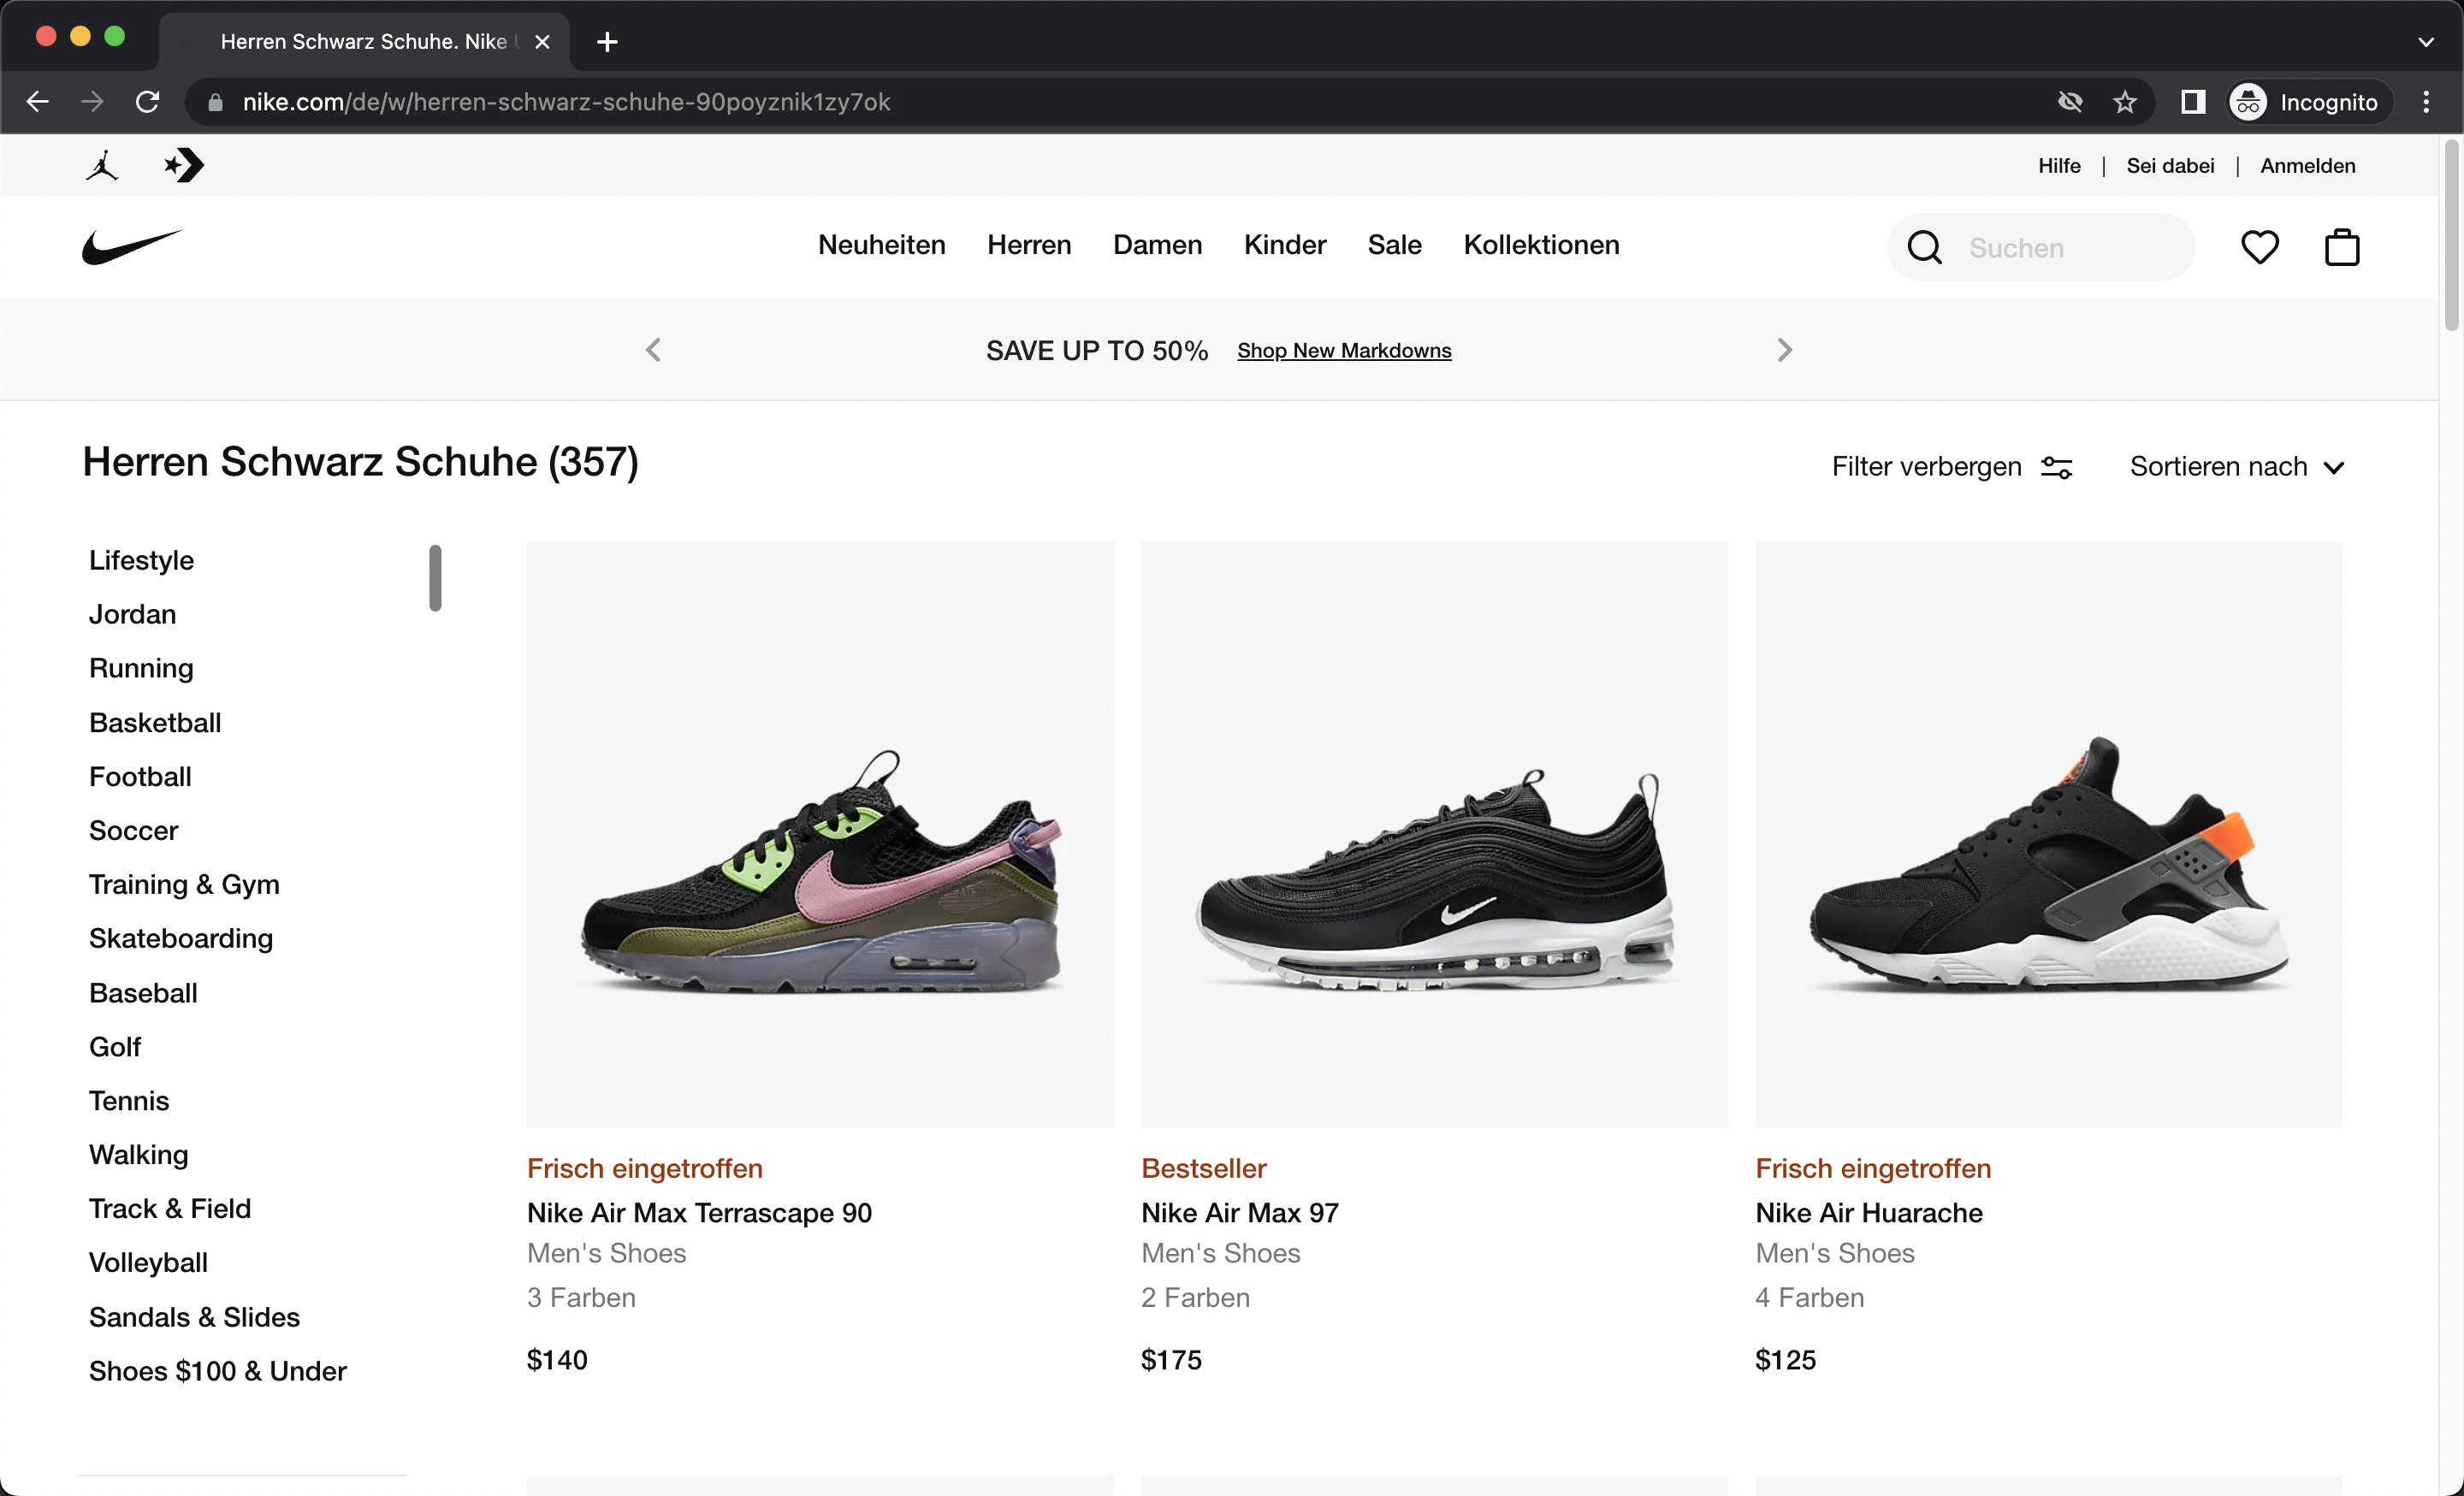
\includegraphics[width=\textwidth]{assets/screenshot_nike_website.png}
  \caption{Nike's Mens Black Sneakers URL full-path}
  \label{fig:nikeMensBlackSneakersUrl}
\end{figure}

In practice, however, not all websites adhere to these guidelines. A good comparison would be how Nike and Lacoste filter their products on their respective websites (See \autoref{fig:nikeMensBlackSneakersUrl} and \autoref{fig:lacosteMensBlackSneakersUrl}). In both of these examples, the user is looking for black sneakers on their respective websites. The figures show that both have different ways of displaying the URL. Nike includes the filters and facets in the URL path, as well as a hash string at the end. Lacoste, on the other hand, stores the classic filter in the URL path and the facets as URL queries, which is the preferred method of utilizing the URL. Lacoste stores the query parameter's value in a JSON format. If the URL is decoded twice, the output would be: \verb;?filters={"searchColorID":"Schwarz"}';.

\begin{figure}[H]
  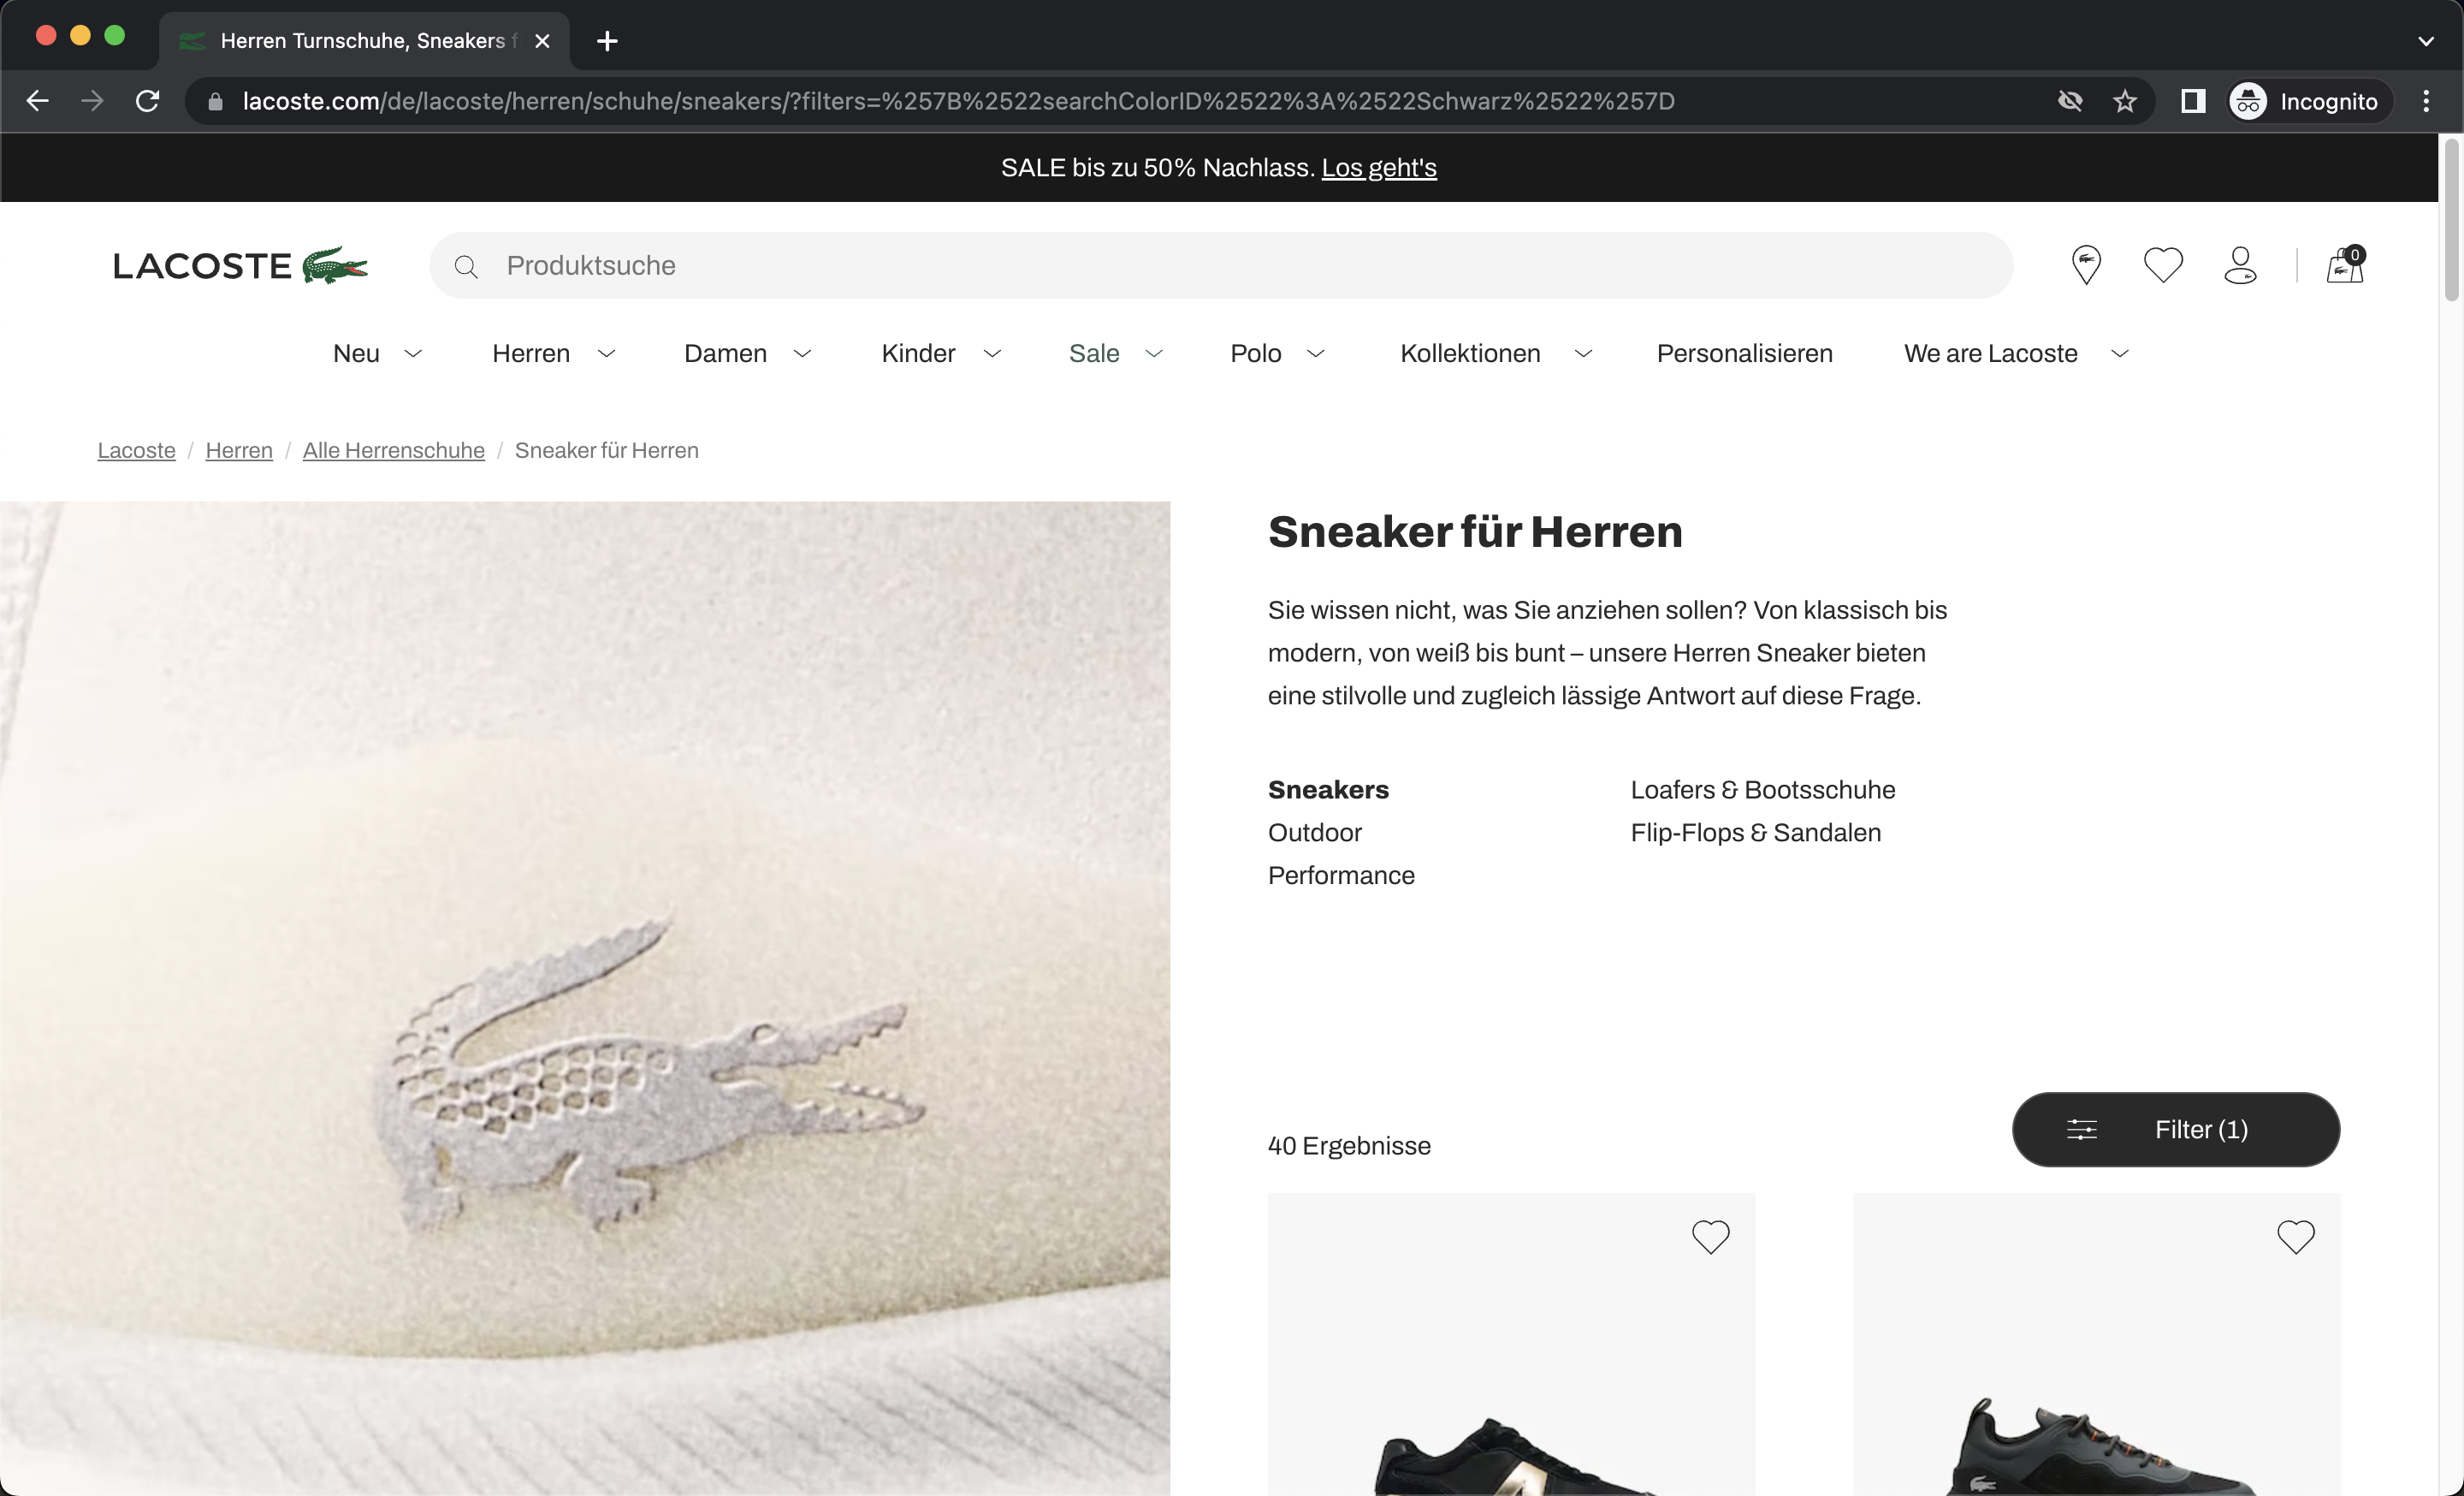
\includegraphics[width=\textwidth]{assets/screenshot_lacoste_website.png}
  \caption{Lacoste's Mens Black Sneakers URL full-path}
  \label{fig:lacosteMensBlackSneakersUrl}
\end{figure}

The solution to this problem would be to save not only the URL's query parameters, but also the path component. These properties should be accessible via the same host name. This solution, however, raises another issue: how to transform the URL so that it can be stored as JSON.

\subsection*{Converting URL to JSON Object}
The URL must be saved as a JSON object in order to count how many times each query parameter for each host is entered. The following is an example of storing a simple URL with only one path and a query parameter:

\noindent\begin{center}
  \url{https://app.marta.de/caregivers?caregiver.germanVerbalProficiency=one,two}
\end{center}

\begin{lstlisting}[language=json, caption={A record example from app.marta.de (JSON)}]
{
  "app.marta.de": [
    {
      "name": "/caregivers",
      "parameters": [
        {
          "count": 1,
          "createdAt": 1660224894790,
          "lastUpdatedAt": 1660224894790,
          "paramKey": "caregiver.germanVerbalProficiency",
          "paramValue": "one,two",
          "uuid": "8006a4a5-482e-4282-940f-569a54fd29ce",
          "version": "0.1.0"
        }
      ],
      "subpaths": []
    }
  ]
}
\end{lstlisting}

Converting such a basic URL to a JSON object is a simple task. The outermost key is host, the inner key is path, and the value is an array of query parameters in JSON format. When converting more complicated URLs on a faceted navigation system as shown in \autoref{fig:lacosteMensBlackSneakersUrl}, a problem arises.

In order to store nested URL path in our data structure, the URL is traversed in a similar manner to directories. For this reason, a recursive helper function is implemented to convert URL pathname to a JSON object. So the aforementioned URL can be saved as follows:

\begin{lstlisting}[language=json, caption={Record with long pathname (JSON)}, label={lst:recordLongPathname}]
{
  "www.lacoste.com": [
		{
			"name": "/de",
			"parameters": [],
			"subpaths": [
				{
					"name": "/lacoste",
					"parameters": [],
					"subpaths": [
						{
							"name": "/herren",
							"parameters": [],
							"subpaths": [
								{
									"name": "/schuhe",
									"parameters": [],
									"subpaths": [
										{
											"name": "/sneakers",
											"parameters": [],
											"subpaths": [
												{
													"name": "/",
													"parameters": [
														{
															"count": 1,
															"createdAt": 1660552042754,
															"lastUpdatedAt": 1660552042754,
															"paramKey": "filters",
															"paramValue": "%7B%22searchColorID%22:%22Schwarz%22%7D",
															"uuid": "8a737280-8feb-4968-a97f-222424eb6c95",
															"version": "0.1.0"
														}
													],
													"subpaths": []
												}
											]
										}
									]
								}
							]
						}
					]
				}
			]
		}
	],
}
\end{lstlisting}

Because the data structure shown in \autoref{lst:recordLongPathname} is quite scalable, visiting another pathname from the same host would not be a problem, as shown in \autoref{lst:recordDifferentPathnames}. This structure allows each subpath to have another subpaths and queries. This structure enables each subpath to contain additional subpaths and queries. If a user visits the URL \url{https://www.lacoste.com/de/lacoste/herren/schuhe?filters=...}, the parameter values are then pushed into the parameters array under the subpath \texttt{/schuhe}.

\begin{lstlisting}[language=json, caption={Record with different pathnames (JSON)}, label={lst:recordDifferentPathnames}]
...
  {
    "name": "/schuhe",
    "parameters": [],
    "subpaths": [
      {
        "name": "/sneakers",
        "parameters": [],
        "subpaths": [
          {
            "name": "/",
            "parameters": [
              {
                "count": 2,
                "createdAt": 1660552137705,
                "lastUpdatedAt": 1660552137705,
                "paramKey": "filters",
                "paramValue": "%7B%22searchColorID%22:%22Schwarz%22%7D",
                "uuid": "5882c1bf-92e8-4e3f-9454-1b6f1acd6dc7",
                "version": "0.1.0"
              }
            ],
            "subpaths": []
          }
        ]
      },
      {
        "name": "/outdoor",
        "parameters": [],
        "subpaths": [
          {
            "name": "/",
            "parameters": [
              {
                "count": 1,
                "createdAt": 1660552464135,
                "lastUpdatedAt": 1660552464135,
                "paramKey": "filters",
                "paramValue": "%7B%22searchColorID%22:%22Schwarz%22%7D",
                "uuid": "31b25e02-9631-4bc1-acda-740c7fb58343",
                "version": "0.1.0"
              }
            ],
            "subpaths": []
          }
        ]
      }
    ]
  }
...
\end{lstlisting}

\begin{lstlisting}[style=ES6, caption={Resursive pathname to JSON function (TypeScript)}]
const recursiveFunc = (
  filters: PathType[],
  paths: Array<string>,
  parameters: Record<string, string | string[]>
) => {
  const element = paths.shift()
  if (typeof element === 'undefined' || element === null) return
  const pathIndex = filters.findIndex((f) => f.name === element)

  if (pathIndex > -1) {
    if (paths.length > 0) {
      recursiveFunc(filters[pathIndex].subpaths, paths, parameters)
    } else {
      filters[pathIndex].parameters = upsertParams(
        filters[pathIndex].parameters,
        parameters
      )
    }
  } else {
    if (paths.length > 0) {
      const newLength = filters.push({
        name: element,
        parameters: [],
        subpaths: []
      })
      recursiveFunc(filters[newLength - 1].subpaths, paths, parameters)
    } else {
      const newParameters = upsertParams([], parameters)
      filters.push({
        name: element,
        parameters: newParameters,
        subpaths: []
      })
    }
  }
}
\end{lstlisting}
